% Chapter 3

\chapter{Estado del Arte} % Main chapter title

\label{Chapter3} % Change X to a consecutive number; for referencing this chapter elsewhere, use \ref{ChapterX}

Los trabajos y estudios ya realizados que están relacionados con nuestra propuesta de proyecto terminal o marcan un precedente a esta, se encuentran en esta sección, con la finalidad de presentar antecedentes, y dejar ver discrepancias y similitudes con estos.\newline

La complejidad que puede representar el realizar un análisis acertado, de una red móvil, ha resultado en la necesidad de realizar simulaciones de estas. En "Análisis de rendimiento en sistemas celulares 4G mediante algoritmos de asignación de recursos (canal, sub-portadoras)" \parencite{Celis2016}, encontramos un proyecto terminal realizado por alumnos de la UPIITA, en el cual se realizó la simulación, bajo el paradigma de eventos discretos, de un sistema celular 4G, enfocando su investigación en distintos esquemas de reúso de frecuencias y calendarizadores para obtener resultados sobre qué combinación de estos y bajo qué condiciones permitían al sistema tener un mayor desempeño. En este proyecto la simulación se llevó a cabo utilizando Matlab, el paradigma de programación fue el de eventos discretos por lo que presenta un buen precedente a nuestro proyecto en la UPIITA y es también un ejemplo de cómo el trabajo de dimensionar los sistemas de comunicación móviles es una necesitad recurrente en cada generación. \newline

Se estudiaron de manera puntual diferentes modelos de sistema que sirvieron de apoyo para fundamentar las bases del proyecto, a continuación se detallan los aspectos más importantes de cada uno:

%----------------------------------------------------------------------------------------
%	SECTION 
%----------------------------------------------------------------------------------------

\section{\textit{'Joint Downlink/Uplink RF Wake-Up Solution for IoT Over Cellular Networks'}}

En \parencite{Kouzayha2018} los autores presentan un modelo de sistema para redes celulares IoT, cuya principal premisa es la implementación de una solución que llamaron \textit{WAKE-UP. }Este sistema despierta por señales de radio frecuencia a los dispositivos IoT, para los que se modeló un estado de sueño profundo.\newline

Esta señal de despertador de RF garantiza la alta capacidad de respuesta del dispositivo cuando se le solicita comunicación y reduce la actividad de escucha inactiva, que consume una parte notable de la energía de la batería. Estos esquemas de activación bajo demanda son particularmente adecuados para aplicaciones de IoT con bajo ciclo de trabajo (por ejemplo, detección de incendios, vigilancia de fallas de máquinas y, en general, todos los escenarios controlados por eventos). \newline

El modelo propuesto en \parencite{Kouzayha2018} sigue un mecanismo similar al \textit{Power Saving Mode} (PSM) definido por la 3GPP (y usado en NB-IoT), coinciden en que los nodos IoT entrarán en un estado de sueño profundo cuando no tengan datos que transmitir, mas sin embargo en el PSM se hace uso de temporizadores para activar al nodo IoT, en contraste con la señal RF de despertador que se plantea aquí.\newline

Este modelo utiliza una geometría estocástica para distribuir en el plano tanto a las estaciones base como a los dispositivos siguiendo un PPP independiente con una densidad espacial distinta tanto para las estaciones base como para los dispositivos, esto lo podemos ver gráficamente en la \textit{Figura~\ref{fig:distribuBS}}:

\begin{figure}[th]
\centering
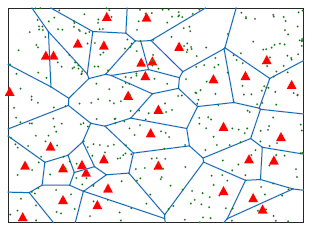
\includegraphics[scale=.8]{Figures/Distribución de estaciones base (triángulos) y dispositivos (puntos)}
\decoRule
\caption[Distribución de estaciones base y dispositivos]{Distribución de estaciones base (triángulos) y dispositivos (puntos)}
\label{fig:distribuBS}
\end{figure}

La principal característica del modelo es la capacidad de los dispositivos de internarse en un estado, propuesto en el modelo, llamado estado de sueño profundo (\textit{deep sleep state) }el cual permitiría tener un ahorro de energía en comparación con el modo de ahorro de energía (\textit{Power Saving Mode, PSM) }propuesto por la 3GPP. \newline

De este estado de sueño profundo\textit{ }a diferencia de tener similitudes con el PSM no se sale de manera periódica cuando se termina un temporizador, sino que la única forma de salir de él es a través de una señal de \textit{wake-up} transmitida desde la estación base que le brinda servicio al nodo que se encuentra en el estado de sueño profundo, siempre y cuando esta señal cuente con la potencia suficiente para activar la circuitería del dispositivo. \newline

Esto trae a escena nuevas consideraciones a tener, debido a que si bien no existe interferencia intercelular en el modelo de \parencite{Kouzayha2018}, el reusó de canal tiene un valor de 1 y las estaciones bases adyacentes utilizan los mismos recursos para intentar despertar a sus propios dispositivos, de manera de que falsos despertares pueden ocurrir entre los dispositivos. Esto se puede apreciar en la Figura~\ref{fig:despertar}.\newline

\begin{figure}[th]
\centering
\includegraphics[scale=1]{Figures/Demostración de un despertar falso y uno correcto}
\decoRule
\caption[Demostración de un despertar falso y uno correcto]{Demostración de un despertar falso y uno correcto}
\label{fig:despertar}
\end{figure}

El artículo propone entonces la implementación de un bloque en la circuitería de los nodos IoT que se encargue de realizar 3 operaciones como se puede apreciar en la Figura~\ref{fig:circuiteria}, el emparejamiento de la red quien reduciría la perdida de transmisión desde la antena e incrementar el voltaje proporcionado al rectificador, el rectificador se encarga de convertir la señal RF en voltaje DC mientras que el detector de ID se encarga de comparar el ID del dispositivo con el de la señal RF.\newline

\begin{figure}[th]
\centering
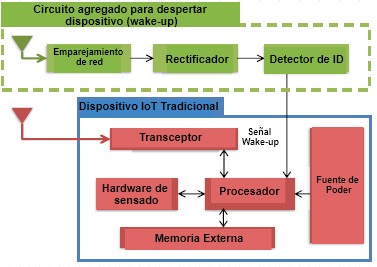
\includegraphics[scale=1]{Figures/Implementación de wake-up RF en la circuitería IoT}
\decoRule
\caption[Implementación de \textit{wake-up} RF en la circuitería IoT]{Implementación de \textit{wake-up} RF en la circuitería IoT}
\label{fig:circuiteria}
\end{figure}

Finalmente se presentan resultados de las probabilidades de falsos y correctos despertares además del ahorro en el consumo de energía reportado en comparación con la opción de PSM.


%----------------------------------------------------------------------------------------
%	SECTION 
%----------------------------------------------------------------------------------------

\section{\textit{'Downlink and uplink non-orthogonal multiple access in a dense wireless network'}}

En \parencite{Zhang2017}, los autores proponen un sistema usando geometría estocástica para modelar un ambiente inalámbrico denso, que admita NOMA tanto en el enlace de subida como en el enlace de bajada; el modelado es analítico y validado por simulación.\newline

Los aspectos generales del sistema considerados en \parencite{Zhang2017} son:
\begin{itemize}
\item  Ambiente denso de múltiples celdas con factor de reuso de 1 con geometría estocástica usando \textit{Poisson Point Process} (PPP) para modelar el despliegue de las BS y UE en un plano Euclidiano 2D.
\end{itemize}

\textbf{Sistema \textit{downlink}}\newline

Los autores consideran un error de propagación SIC durante el proceso de decodificación por parte del UE. Se hace uso de dos esquemas de emparejamiento de usuario: aleatorio y selectivo.\newline

\begin{enumerate}
\item  Cuando el agrupamiento es aleatorio, los UE son seleccionados aleatoriamente.
\item  Cuando el agrupamiento es selectivo, el primer UE deberá tener una relación señal-interferencia más ruido (SINR) por encima del umbral T1 y el segundo UE tiene un SINR por debajo del umbral T2, T2 $\mathrm{\le}$ T1.
\end{enumerate}

En ambos esquemas de emparejamiento, el UE con una mejor ganancia de canal normalizada se denota como UE1 y el UE con una peor ganancia de canal normalizada se denota como UE2.\newline

Se optó por una estrategia de asignación de potencia fija, donde la potencia de enlace de bajada asignada a un UE está predefinida y permanece sin cambios.\newline


\begin{figure}
\centering
\begin{minipage}{.45\linewidth}
  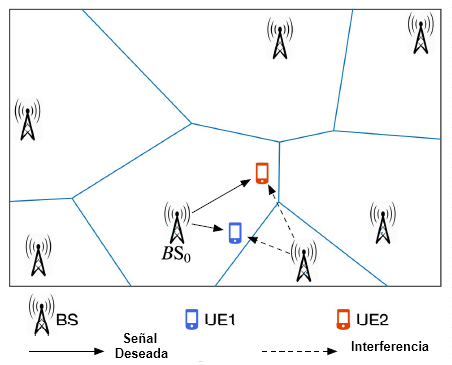
\includegraphics[width=\linewidth]{Modelo de sistema para el sistema de enlace descendente NOMA}
  \captionof{figure}{Modelo de sistema para el sistema de enlace descendente NOMA}
  \label{fig:img1}
\end{minipage}
\hspace{.05\linewidth}
\begin{minipage}{.45\linewidth}
  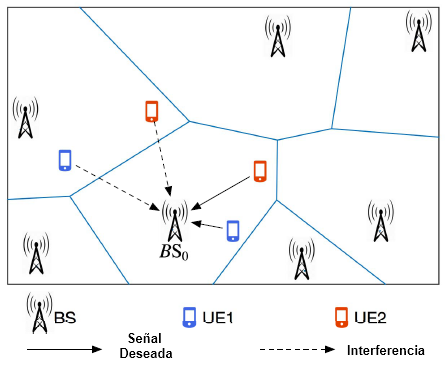
\includegraphics[width=\linewidth]{Modelo de sistema para el sistema de enlace ascendente NOMA}
  \captionof{figure}{Modelo de sistema para el sistema de enlace ascendente NOMA}
  \label{fig:img2}
\end{minipage}
\end{figure}

Las ganancias implementan el desvanecimiento de Rayleigh entre BS0 y UEi. La ganancia de desvanecimiento Rayleigh entre BS y UE sigue una distribución exponencial con media 1 y se distribuye de forma independiente e idéntica (i.i.d.)\newline
Para todos los UE, ${ri}$ se distribuye de forma independiente e idéntica (i.i.d.) con una función de densidad de probabilidad (pdf) dada.\newline
En el enlace Descendente,se agregan perdidas por trayectoria con un exponente de pérdida y se calcula la interferencia entre celdas cumulativa de todas las bases adyacentes.\newline
En el enlace Ascendente, la interferencia inter-celdas proviene de todos los otros UEs que comparten la misma sub-banda. \textit{[Véanse Figuras~\ref{fig:img1}, \ref{fig:img2}]}


%----------------------------------------------------------------------------------------
%	SECTION 
%----------------------------------------------------------------------------------------

\section{\textit{'NOMA Aided Narrowband IoT for Machine Type Communications With User Clustering'}}


%----------------------------------------------------------------------------------------
%	SECTION 
%----------------------------------------------------------------------------------------

\section{}

\myworries{TODO: ACTUALIZAR estado del arte de acuerdo a los articulos nuevos que tomamos en consideración}\newline